\documentclass[conference]{IEEEtran}
\usepackage[utf8]{inputenc}
\usepackage[spanish,english]{babel}

\usepackage{graphicx}
\usepackage{float}

\usepackage[style=ieee]{biblatex}
\usepackage{csquotes}
\addbibresource{referencias.bib}

\begin{document}

%%%%%%%%%%%%%%%%%%%% PORTADA %%%%%%%%%%%%%%%%%%%%%%%%%%%%%%
\begin{titlepage}

\centering

\includegraphics[scale=0.6]{una.png}\\[10mm]

\textbf{
    {\Large Facultad de Ciencias Exactas y Naturales\\[3mm]
    Escuela de Informática y Computación\\[3mm]
    Ingeniería en Sistemas de Información\\[3mm]
    Paradigmas de Programación}\\[15mm]
    {\LARGE Algoritmos para la generación y solución eficiente de Sudokus}\\[15mm]
}

\large{Integrantes:}\\[3mm]

\begin{minipage}{0.4\textwidth}
\begin{flushleft} \large
\centering
    Andrey Arguedas Espinoza\\
    \texttt{4-0231-0255}\\
    Daniela Armas Sánchez\\
    \texttt{4-0232-0156}\\
\end{flushleft}
\end{minipage}
~
\begin{minipage}{0.4\textwidth}
\begin{flushleft} \large
\centering
    Michael Chen Wang\\
    \texttt{1-1629-0538}\\
    Kimberly Olivas Delgado\\
    \texttt{1-1683-0271}\\
\end{flushleft}
\end{minipage}\\[15mm]

\large{Profesor: \\[3mm] Carlos Loría Sáenz}\\[15mm]

\large {II Ciclo, 2017}

\end{titlepage}
\clearpage


\title{Algoritmos para la generación y solución eficiente de Sudokus}
\author{Andrey Arguedas, Daniela Armas, Michael Chen, Kimberly Olivas}
\maketitle

%%%%%%%%%%%%%%%%%%%% RESUMEN %%%%%%%%%%%%%%%%%%%%%%%%%%%%%%
\begin{otherlanguage}{spanish}
\begin{abstract}
El presente documento busca que el lector se familiarice con conceptos básicos del juego matemático Sudoku y con cómo este puede ser solucionado y generado mediante algoritmos y técnicas computacionales. Esto se lleva a cabo por medio de la resolución de un proyecto cuyo objetivo es el desarrollo de una aplicación web que permita jugar al Sudoku.

Para dicho proyecto se requirió, aparte de nuevos conocimientos técnicos, la búsqueda y comprensión de las principales características y reglas del juego. Posteriormente, se debió investigar acerca de algoritmos, técnicas o heurísticas que facilitan la solución o generación de un tablero de Sudoku, de las cuales se seleccionaron el \textit{backtrack}, \textit{naked single} y \textit{hidden single}. 
\end{abstract}
\end{otherlanguage}

%%%%%%%%%%%%%%%%%%%% INTRODUCCIÓN %%%%%%%%%%%%%%%%%%%%%%%%%
\section{Introducción}
El objetivo del presente proyecto es la implementación de la lógica y la arquitectura de un juego de Sudoku en una aplicación web utilizando un \textit{stack} MEAN (Mongo, Express, Angular y Node), poniendo en práctica la programación funcional y orientada a objetos. 

El Sudoku es un juego matemático inventado a finales de los años 70 basado en un sistema de probabilidades para representar una serie de números sin repetir inventado por Leonhard Euler de Basilea en el siglo XVIII \cite{sudokuWiki}. 
Consiste en una cuadrícula, por lo general de 9x9, dividida en sub-cuadrículas de 3x3, la cual se debe llenar con números del 1 al 9 en cada columna, cada fila y cada sub-cuadrícula, sin repeticiones ni conflictos en los tres casos. La cuadrícula inicialmente debe poseer al menos 17 “pistas” o números ubicados en las casillas del juego, los cuales no pueden ser cambiados por el jugador. Dichas reglas se debieron tomar en cuenta a la hora de implementar los métodos y algoritmos principales de solución y creación.
 
Para ello, se debió realizar una investigación y selección de algoritmos eficientes. Se eligió el \textit{backtracking} como algoritmo principal para la solución de sudokus y, además, las técnicas de \textit{hidden single} y \textit{naked single} que ayudan a eliminar opciones de números en cada casilla. Ambas técnicas, al ser combinadas con un algoritmo de solución como lo es el \textit{backtrack}, se vuelven más eficientes para el programa, mejoran sustancialmente el tiempo de corrida del algoritmo y además logran que se realicen menos llamadas recursivas que resultan siendo muy costosas para la máquina encargada de computar dicho algoritmo.


%%%%%%%%%%%%%%%%%%%% DESARROLLO %%%%%%%%%%%%%%%%%%%%%%%%%%%
\section{Algoritmos y técnicas}
Los algoritmos del proyecto fueron seleccionados según su capacidad de solución o generación de un sudoku. Los mismos se explican a continuación.

\subsection{Algoritmos y técnicas para solución}
\subsubsection{Backtrack}
El algoritmo de \textit{backtrack} o “vuelta atrás” es un tipo de búsqueda de fuerza bruta utilizado para encontrar soluciones a problemas que satisfacen restricciones \cite{vueltaAtras}. Dicha técnica hace una búsqueda en profundidad ya que explora completamente una rama buscando la solución antes de pasar a la siguiente rama.

En grandes rasgos, el algoritmo de \textit{backtracking} usado para resolver el sudoku, visita en orden cada una de las celdas vacías y las va rellenando secuencialmente con un número del 1 al 9 según lo permitan las restricciones. 
Si el número colocado en una celda es válido, el algoritmo se mueve a la siguiente celda y le asigna el primer número de la secuencia. Si el número es inválido, es decir se repite en la fila, columna o sub-cuadrícula de esta celda, el algoritmo le asigna el siguiente número de la secuencia. Si se han probado los 9 dígitos de la secuencia y ninguno cumple con las restricciones, el algoritmo deja esta celda en blanco y retrocede a la celda anterior, aumentando en uno el valor de esta celda. Este proceso se repite hasta que todas las celdas tengan un número válido, es decir hasta que el algoritmo haya resuelto las 81 celdas \cite{sudokuSolving}.

En las figuras~\ref{fig:backtrack1} y~\ref{fig:backtrack2} se puede observar cómo el algoritmo implementado logra resolver un sudoku.

\begin{otherlanguage}{spanish}
\begin{figure}[H]
\centering
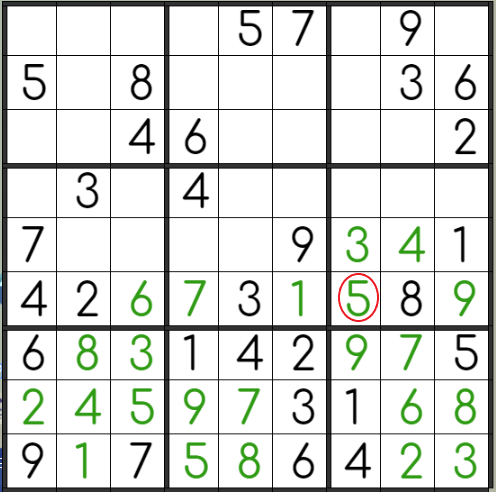
\includegraphics[width=0.4\textwidth]{backtrack1.png}
\caption{\label{fig:backtrack1}Proceso de backtracking.}
\end{figure}
\end{otherlanguage}

En la figura~\ref{fig:backtrack1} se muestra el algoritmo en proceso, y se resalta una casilla con el número 5, mientras que en la figura~\ref{fig:backtrack2}, que muestra el sudoku ya resuelto, este número cambia por el 6, lo cual representa que el algoritmo en un punto tuvo que devolverse a esa casilla y cambiar el valor para seguir probando opciones.

\begin{otherlanguage}{spanish}
\begin{figure}[H]
\centering
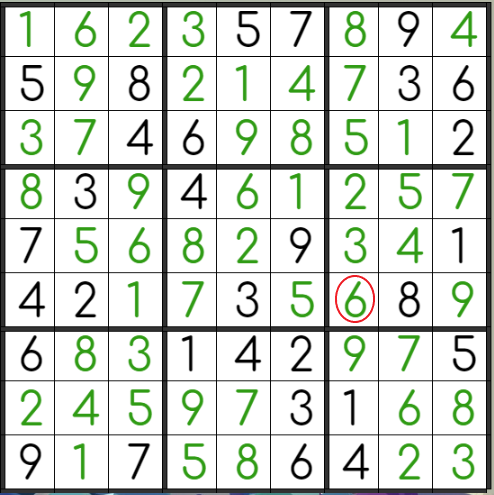
\includegraphics[width=0.4\textwidth]{backtrack2.png}
\caption{\label{fig:backtrack2}Solución con backtrack.}
\end{figure}
\end{otherlanguage}

El \textit{backtrack} tiene la ventaja de garantizar una solución para el sudoku sin importar la dificultad que presente, sin embargo, posee la desventaja de que el tiempo de resolución puede ser muy lento ya que verifica todas las posibles soluciones, además de que la pila de llamados recursivos podría llegar a alcanzar un tamaño bastante extenso debido a la cantidad de veces que se debe implementar el \textit{backtrack}. Otra desventaja es que se pueden construir sudokus que trabajen en contra del \textit{backtrack}, ciertos heurísticos como dar pocas pistas o acomodarlas de cierta manera pueden aumentar la dificultad del sudoku para ser resuelto por esta técnica.


\subsubsection{Naked Single}
La técnica “único desnudo” o \textit{naked single} es una de las más simples para la solución de sudokus. 

Consiste en determinar los posibles valores de una celda vacía examinando los valores de las celdas llenas en la fila, columna y sub-cuadrícula de esta celda. Si al final de la revisión, la celda vacía tiene un único posible valor, éste debe ser el valor de la celda \cite{nakedSolving}.

Considerando las “pistas” del sudoku de la figura~\ref{fig:naked1}, se pueden resolver algunas celdas haciendo uso de esta técnica. Por ejemplo, después de revisar su fila, columna y sub-cuadrícula, se puede determinar que la sétima celda de la primera fila es \textit{naked single}.

\begin{otherlanguage}{spanish}
\begin{figure}[H]
\centering
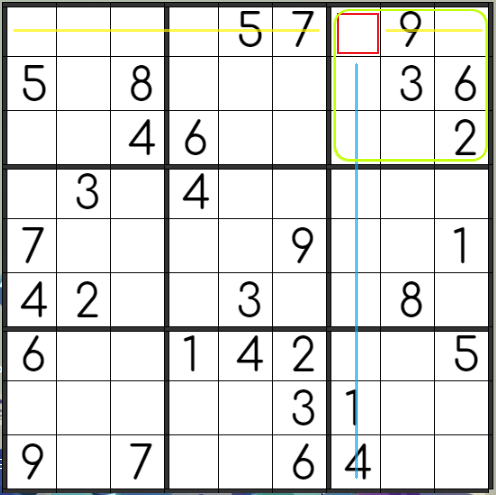
\includegraphics[width=0.4\textwidth]{nakedsingle1.png}
\caption{\label{fig:naked1}Análisis de opciones con Naked Single.}
\end{figure}
\end{otherlanguage}

Se llega a esta conclusión debido a que dicha celda termina con un único valor. Inicialmente la celda tiene los 9 posibles valores. Sin embargo, la sub-cuadrícula elimina de las posibilidades los números 2, 3, 6 y 9. Por otro lado se descartan los números 1 y 4 por la columna, y 5 y 7 por la fila. Por lo tanto, al final de la revisión el valor de dicha celda debe ser un 8, como se observa en la figura~\ref{fig:naked2}.

\begin{otherlanguage}{spanish}
\begin{figure}[H]
\centering
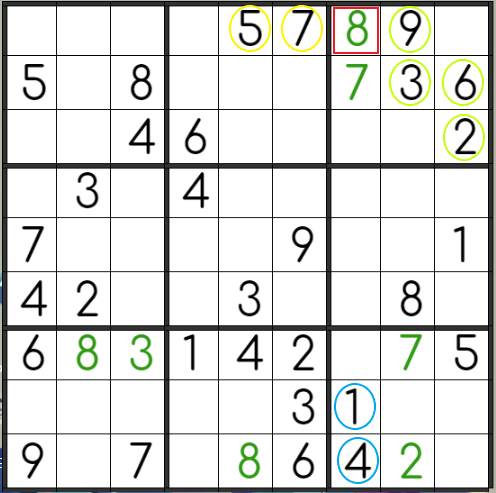
\includegraphics[width=0.4\textwidth]{nakedsingle2.png}
\caption{\label{fig:naked2}Selección de valor con Naked Single.}
\end{figure}
\end{otherlanguage}

Es importante destacar que cada vez que se encuentre una celda con sólo un posible valor, este se debe eliminar de las posibilidades de todas las celdas de su fila, columna y sub-cuadrícula. Esto quiere decir que, si el valor de una celda queda \textit{naked single}, puede desencadenar que muchas otras celdas también queden con valores únicos.

Su desventaja es que sólo es capaz de resolver sudokus completos si son de muy baja dificultad. Sin embargo, puede ser de utilidad para encontrar una solución parcial del sudoku. De modo que queden algunas celdas resueltas, facilitando así que otra técnica o algoritmo lo solucione en su totalidad.

\subsubsection{Hidden Single}
La técnica de resolución “único oculto” o \textit{hidden single} también es bastante sencilla pero resulta más eficaz.

Utilizando esta técnica se determinan los posibles valores de todas las celdas vacías en una fila, columna y sub-cuadrícula determinada. Si un posible valor aparece en sólo una celda de una fila y columna que se intersecan o en la sub-cuadrícula que pertenece dicha celda, entonces ese debe ser el valor de la celda \cite{hiddenSolving}. Se dice que es oculto porque éste único valor se encuentra dentro de la celda junto con otros candidatos \cite{individual}.

En la figura~\ref{fig:hidden1} se puede observar que la cuarta celda de la primera fila es \textit{hidden single}. Para determinar esto, se definen los posibles valores de cada celda y posteriormente se evalúan dicShos valores por “categorías” o grupos correspondientes a la fila, columna o sub-cuadrícula. En este caso en particular, se verifican los posibles valores de la sub-cuadrícula a la que pertenece la celda para hallar el único valor que no es candidato en ninguna otra celda.

\begin{otherlanguage}{spanish}
\begin{figure}[H]
\centering
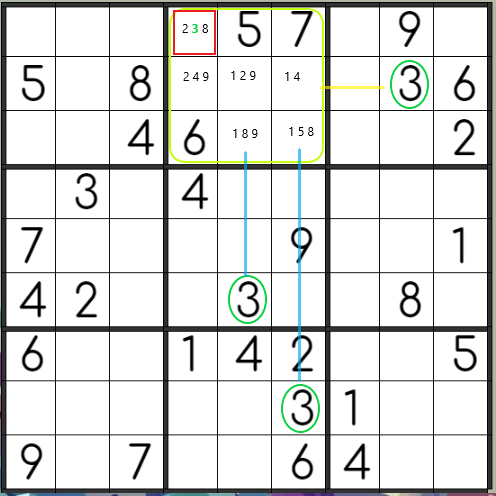
\includegraphics[width=0.4\textwidth]{hiddensingle1.png}
\caption{\label{fig:hidden1}Lógica de selección de un valor con Hidden Single}
\end{figure}
\end{otherlanguage}

Como se muestra en la figura~\ref{fig:hidden1}, la cuarta celda de la primera fila es la única de toda la segunda sub-cuadrícula que posee el número 3 como candidato, por lo que este debe ser el valor definitivo de la celda. Ver figura~\ref{fig:hidden2}. 

\begin{otherlanguage}{spanish}
\begin{figure}[H]
\centering
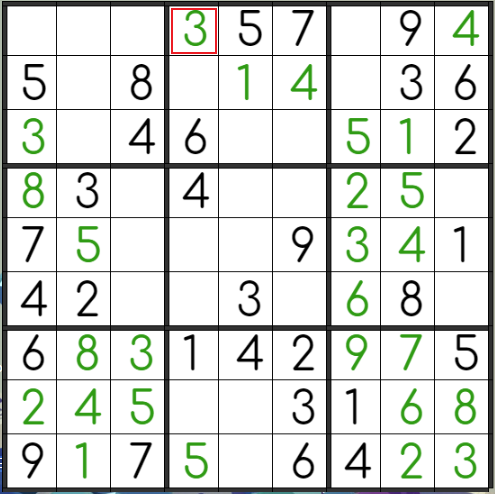
\includegraphics[width=0.4\textwidth]{hiddensingle2.png}
\caption{\label{fig:hidden2}Valor seleccionado con Hidden Single.}
\end{figure}
\end{otherlanguage}

Al igual que con la técnica \textit{naked single}, conforme se vayan encontrando los valores correctos de las celdas se van actualizando los posibles valores de todas las celdas vecinas (es decir, de su misma fila, columna o sub-cuadrícula), lo que provocaría que algunas otras celdas puedan quedar \textit{hidden single}.

Esta técnica es capaz de solucionar por completo sudokus de dificultad media. Sin embargo es mayormente utilizado en conjunto con otras heurísticas para generar un algoritmo de resolución más eficiente.

\subsection{Algoritmo de generación}
Se utiliza como base la idea de \textit{backtracking} mencionada anteriormente, sin embargo, se le realizan algunos cambios a la técnica que permitan la generación completa de un sudoku.

En este caso en particular, el algoritmo visita en orden cada una de las celdas vacías y las va rellenando aleatoriamente con un número del 1 al 9. Si el número colocado es válido, el algoritmo elige un número aleatorio de los 9 candidatos y se lo asigna a la siguiente celda. Sin embargo, si el número es inválido, es decir se repite en la fila, columna o sub-cuadrícula de esta celda, el algoritmo le asigna otro número aleatorio que no haya sido utilizado antes para dicha celda. De igual forma si se acaban las 9 posibilidades para la celda, se retrocede a la anterior y se repite el proceso.

Una vez que se genera por completo el sudoku, en otras palabras, cuando todas las 81 celdas contienen números válidos, el algoritmo elige únicamente de 17 a 23 celdas para mostrar las “pistas” del sudoku, dejando las demás vacías para ser completadas por el jugador. En la figura \ref{fig:generate} se muestra el resultado final de un sudoku elaborado por dicho algoritmo.

\begin{otherlanguage}{spanish}
\begin{figure}[H]
\centering
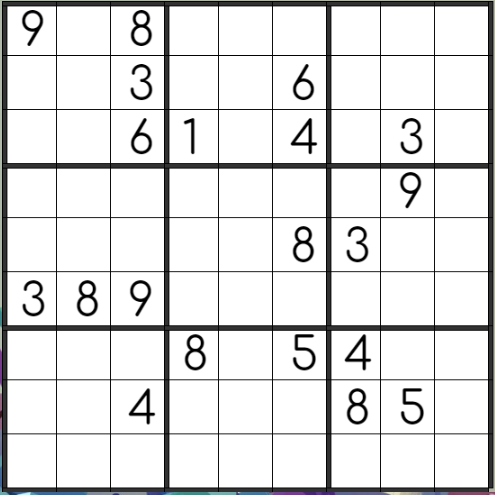
\includegraphics[width=0.4\textwidth]{generate.png}
\caption{\label{fig:generate}Sudoku generado por el algoritmo.}
\end{figure}
\end{otherlanguage}

Cabe destacar que los sudokus no se generan con una dificultad establecida, ya que no existe algún algoritmo que pueda identificar la dificultad de un sudoku.

\section{Dificultad de un sudoku}

La dificultad de un sudoku depende de la cantidad de pistas que posea y las casillas en las que sean ubicadas. A pesar de que los sudokus generados por nuestro algoritmo no poseen dificultades establecidas, en la aplicación se brinda la opción de elegir sudokus por dificultad (fácil, media y difícil), los cuales fueron obtenidos previamente de un sitio llamado Web Sudoku en el que se crearon y calificaron  \cite{websudoku}. Los mismos se cargan en la base de datos de la aplicación para poder ser utilizados y resueltos por el jugador.

%%%%%%%%%%%%%%%%%%%% CONCLUSIONES %%%%%%%%%%%%%%%%%%%%%%%%%
\section{Conclusiones}
Cuando se tiene un problema combinatorio como lo es un sudoku, el \textit{backtrack} por sí solo no es la mejor solución, ya que, a pesar de ser un algoritmo que resuelve cualquier tipo de sudoku, el tiempo que tarda es relativo pues depende de la dificultad del mismo, lo cual no es totalmente eficiente. Por lo tanto, es muy importante la utilización de heurísticos para mejorar los algoritmos, que en este caso fueron las técnicas \textit{hidden single} y \textit{naked single}, las cuales mejoraron significativamente la capacidad de resolución del \textit{backtrack}.

Además de la lógica que conlleva la implementación de los métodos y algoritmos del proyecto, se obtuvo un gran aprendizaje en el ámbito técnico, donde se utilizaron nuevas tecnologías y herramientas tales como MongoDB y Mongoose, correspondientes a la base de datos, Node.js siendo un entorno de ejecución del lenguaje de programación Javascript, y Angular 4 para el desarrollo de la aplicación.

Asimismo, se reforzó el uso y comprensión del concepto de promesas y de la programación funcional orientada al estándar ES6 de Javascript, así como el concepto de observables que implementa Angular, librerías gráficas como P5.JS y conocimiento en ambientes de \textit{cloud} como Heroku.

%%%%%%%%%%%%%%%%%%%% REFERENCIAS %%%%%%%%%%%%%%%%%%%%%%%%%%
\begin{otherlanguage}{spanish}
\printbibliography %Prints bibliography
\end{otherlanguage}

\end{document}
